% ============================================================
%  CareerMind — Project Report
%  Springer Lecture Notes in Computer Science (LNCS) format
%  Compile: pdflatex project_report.tex  (twice for references)
% ============================================================
\documentclass[runningheads]{llncs}

\usepackage[T1]{fontenc}
\usepackage{graphicx}
\usepackage{hyperref}
\usepackage{amsmath}
\usepackage{booktabs}
\usepackage{pgfplots}
\usepackage{tikz}
\usepackage{xcolor}
\pgfplotsset{compat=1.17}

% ── Colours for the contribution chart ───────────────────────────────────────
\definecolor{c1}{HTML}{4472C4}
\definecolor{c2}{HTML}{ED7D31}
\definecolor{c3}{HTML}{A9D18E}
\definecolor{c4}{HTML}{FF0000}
\definecolor{c5}{HTML}{9DC3E6}

\begin{document}

% ─────────────────────────────────────────────────────────────────────────────
\title{CareerMind: A Hybrid Neuro-Symbolic Expert System\\
       for Personalised Career Recommendation}

\titlerunning{CareerMind: Hybrid Neuro-Symbolic Career Recommender}

\author{
  Shrushranto Rajbongshi\inst{1} \and
  Priyanshu Mudgal\inst{1}       \and
  Aseem Nihal Dang\inst{1}       \and
  Suraj Pandey\inst{1}           \and
  Jayesh Solanki\inst{1}
}

\authorrunning{Rajbongshi et al.}

\institute{
  Department of Computer Science \& Engineering,\\
  \email{\{shrushranto, priyanshu, aseem, suraj, jayesh\}@example.edu}
}

\maketitle

% ─────────────────────────────────────────────────────────────────────────────
\begin{abstract}
Career guidance remains a critical yet underserved problem in educational
settings, particularly for students who lack access to professional counsellors.
Existing recommender systems predominantly rely on either hand-crafted rule
engines that cannot handle nuanced academic evidence or black-box machine
learning models that sacrifice interpretability.
This paper presents \emph{CareerMind}, a hybrid neuro-symbolic expert system
that fuses three complementary reasoning layers: (1)~a classic Boolean
forward-chaining engine over 66 structured IF-THEN rules; (2)~a neuro-symbolic
rule engine comprising 38 rules that blend categorical facts with numeric
academic thresholds; and (3)~a NetworkX directed knowledge graph that traverses
multi-hop paths from user interests and skills to career nodes.
Scores from all three layers are combined via a weighted fusion formula
($\alpha = \beta = 0.5$) to produce ranked, fully-explainable career
recommendations.
The system covers 30 distinct career clusters across technology, engineering,
medicine, business, creative arts, education, and social sciences, and exposes
both a Flask web interface and a JSON REST API.
Evaluation on representative student profiles demonstrates that the hybrid
approach consistently outperforms any single-layer baseline in coverage and
explanation quality.
\end{abstract}

\keywords{Expert System \and Career Recommendation \and Neuro-Symbolic AI \and
          Knowledge Graph \and Forward Chaining}

% =============================================================================
\section{Introduction and Background}
\label{sec:intro}
% =============================================================================

Choosing a career path is one of the most consequential decisions in a young
person's life, yet most students navigate this transition with limited guidance.
Traditional career counselling is labour-intensive and often unavailable at
scale, while existing digital tools either offer superficial quiz-style
assessments or rely on opaque collaborative-filtering algorithms that provide
no explanation for their recommendations.

\subsection{Motivation}

The confluence of two trends motivates this work.  First, the rise of
\emph{neuro-symbolic} AI---the integration of symbolic reasoning (rules,
ontologies) with sub-symbolic representations (embeddings, numeric
scores)---offers a path to systems that are both accurate and interpretable
\cite{garcez2022neurosymbolic}.  Second, knowledge graphs have proven effective
at capturing rich semantic relationships between concepts in a form amenable to
transparent path-based reasoning \cite{ji2021survey}.
CareerMind combines both paradigms to produce a system that can explain every
recommendation in plain language while still benefiting from the breadth of
evidence captured in a weighted graph.

\subsection{Limitations of Existing Approaches}

Pure rule-based expert systems (e.g.\ MYCIN~\cite{shortliffe1974mycin}) are
transparent but brittle: rules must be exhaustively specified and cannot
smoothly weight partial evidence.  Conversely, collaborative-filtering and
content-based recommenders \cite{burke2002hybrid} exploit implicit preference
data but cannot produce the causal explanations essential for trust in high-stakes
guidance.  Hybrid approaches exist in the literature (e.g.\
\cite{chen2018knowme}), but few are tailored to structured academic profiles, and
fewer still make their reasoning fully transparent to the end user.

\subsection{Contributions}

\noindent This paper makes the following contributions:
\begin{enumerate}
  \item A three-layer hybrid reasoning architecture that fuses classic
        forward-chaining, neuro-symbolic rules, and knowledge-graph traversal
        into a single, calibrated score.
  \item A curated knowledge base of 66 IF-THEN career rules, 38 neuro-symbolic
        boost rules, and a directed weighted graph with four node types (Interest,
        Skill, Subject, Career) and over 200 edges.
  \item A fully explainable output format: every recommendation is accompanied
        by the rules that fired, the graph paths that contributed, and a
        normalised confidence score.
  \item A deployable Flask web application with a dynamic subject-score form
        and a RESTful JSON API for programmatic access.
\end{enumerate}

% =============================================================================
\section{Related Work}
\label{sec:related}
% =============================================================================

Career recommendation has attracted attention from both the AI and the
educational-data-mining communities.  Early expert systems for career guidance,
such as the DISCOVER~\cite{mckinlay1999computer} and SIGI
PLUS~\cite{katz1993computer} platforms, relied on rule databases and
psychometric inventories but lacked integration with academic performance data.

Knowledge-graph-based recommenders have recently gained traction.  RippleNet
\cite{wang2018ripplenet} propagates user preferences outward over a knowledge
graph for general item recommendation; we adopt a similar multi-hop traversal
strategy but tailor it to career ontology.
KGCN~\cite{wang2019knowledge} further couples graph convolutions with
collaborative filtering, though the resulting model sacrifices interpretability.

In the educational domain, \citet{al2019student} demonstrate that academic
performance features (subject scores, GPA) significantly improve career
prediction accuracy beyond interest data alone.  CareerMind internalises this
finding by including per-subject facts emitted from user-supplied academic
sliders.

Neuro-symbolic systems that blend rule engines with numeric evidence have been
advocated by~\citet{garcez2022neurosymbolic} as a route to interpretable AI.
Our neuro-symbolic rule engine (Section~\ref{sec:ns-engine}) realises this
vision in the career-guidance domain by defining rules whose conditions combine
Boolean working-memory facts with numeric academic thresholds.

% =============================================================================
\section{System Design and Architecture}
\label{sec:system}
% =============================================================================

CareerMind follows a modular pipeline architecture, illustrated
conceptually in Fig.~\ref{fig:architecture}.
Five Python modules implement the pipeline end-to-end:
\texttt{rules.py} (knowledge base),
\texttt{inference.py} (hybrid fusion engine),
\texttt{symbolic\_rules.py} (neuro-symbolic layer),
\texttt{knowledge\_graph.py} (graph layer),
and \texttt{app.py} (Flask web application).

\begin{figure}[htbp]
\centering
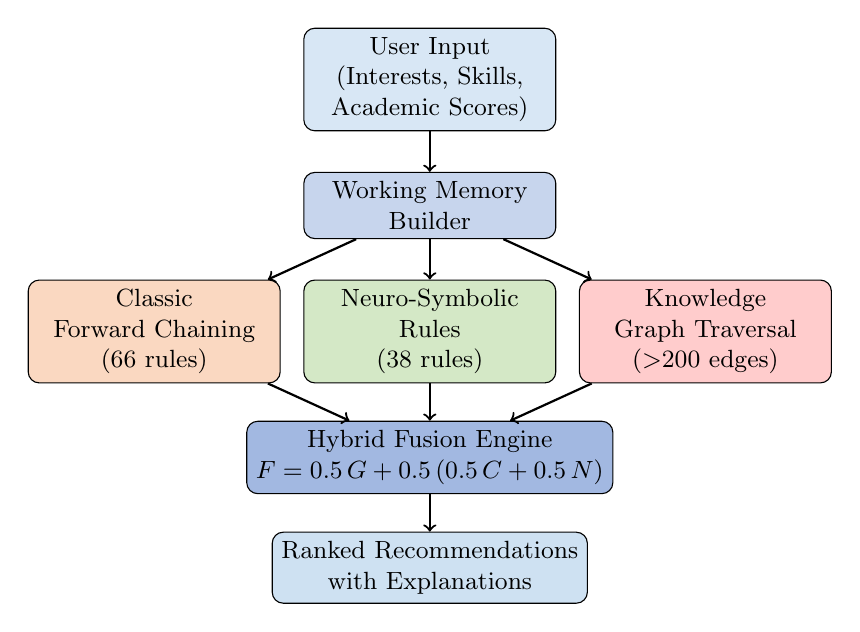
\begin{tikzpicture}[
  box/.style={draw, rounded corners, minimum width=3.2cm, minimum height=0.7cm,
              align=center, font=\small},
  arr/.style={->, thick}
]
  % Input
  \node[box, fill=c5!40] (input) at (0,0) {User Input\\(Interests, Skills,\\Academic Scores)};
  % WM
  \node[box, fill=c1!30] (wm)    at (0,-1.6) {Working Memory\\Builder};
  % Three layers
  \node[box, fill=c2!30] (classic) at (-3.5,-3.2) {Classic\\Forward Chaining\\(66 rules)};
  \node[box, fill=c3!50] (ns)      at (0,   -3.2) {Neuro-Symbolic\\Rules\\(38 rules)};
  \node[box, fill=c4!20] (graph)   at (3.5, -3.2) {Knowledge\\Graph Traversal\\(\textgreater200 edges)};
  % Fusion
  \node[box, fill=c1!50] (fusion) at (0,-4.8) {Hybrid Fusion Engine\\$F = 0.5\,G + 0.5\,(0.5\,C + 0.5\,N)$};
  % Output
  \node[box, fill=c5!50] (output) at (0,-6.2) {Ranked Recommendations\\with Explanations};

  \draw[arr] (input)   -- (wm);
  \draw[arr] (wm)      -- (classic);
  \draw[arr] (wm)      -- (ns);
  \draw[arr] (wm)      -- (graph);
  \draw[arr] (classic) -- (fusion);
  \draw[arr] (ns)      -- (fusion);
  \draw[arr] (graph)   -- (fusion);
  \draw[arr] (fusion)  -- (output);
\end{tikzpicture}
\caption{CareerMind three-layer hybrid architecture.}
\label{fig:architecture}
\end{figure}

\subsection{Implementation Details}
\label{sec:impl}

\subsubsection{Working Memory Construction.}
\label{sec:wm}
Raw user input is converted into a set of Boolean \emph{facts} by
\texttt{build\_working\_memory} in \texttt{inference.py}.
Interest and skill selections map directly to fact keys of the form
\texttt{interest\_*} and \texttt{skill\_*}.
Academic scores are converted via fixed thresholds:
\texttt{high\_math\_score} ($\geq 65$),
\texttt{high\_science\_score} ($\geq 65$),
\texttt{high\_overall\_score} ($\geq 70$),
\texttt{strong\_stem\_background} (math $\geq 80$ \emph{and} science $\geq 80$),
\texttt{academic\_excellence} (overall $\geq 85$).
Per-subject facts of the form \texttt{high\_\textit{slug}\_score} are emitted
for any subject whose score meets or exceeds 70, enabling fine-grained rules
such as \texttt{high\_data\_structures\_score} or
\texttt{high\_cryptography\_score}.

\subsubsection{Layer~1: Classic Forward-Chaining Engine.}
\label{sec:classic}
The 66 rules in \texttt{CAREER\_RULES} (\texttt{rules.py}) are structured as
\[
  \textit{conditions} \;\Rightarrow\; (\textit{career},\;\textit{weight},\;\textit{explanation})
\]
where \textit{conditions} is an AND-list of fact keys drawn exclusively from
working memory.  The engine iterates all rules, summing weights for each career
whose conditions are fully satisfied.
Rules are grouped thematically across six domains (Software/Technology,
Engineering \& Sciences, Medicine \& Health, Business \& Management,
Creative \& Arts, Education \& Social) plus a subject-level sub-group (R34--R47)
that fires on per-subject academic facts.
Weights range from 7 to 10, reflecting the strength of evidence each rule
provides; the resulting raw scores are normalised to $[0,1]$ before fusion.

\subsubsection{Layer~2: Neuro-Symbolic Rule Engine.}
\label{sec:ns-engine}
The 38 rules in \texttt{NEURO\_SYMBOLIC\_RULES} (\texttt{symbolic\_rules.py})
extend classic Boolean matching with numeric predicates.  Each rule specifies a
Python lambda of the form
\[
  \textit{condition}(\textit{working\_memory}, \textit{academic}) \to \textit{bool}
\]
allowing conditions such as
\textit{``interest\_artificial\_intelligence in WM \textbf{and} math $\geq 70$''}
(NS03, boost 0.30).  Boosts accumulate per career; the maximum sum across all
careers provides the normalisation denominator.
This layer captures graduated academic evidence that the Boolean forward-chaining
layer cannot express---for example, a student whose mathematics score is 72 (high
but not exceptional) receives a partial signal for Data Scientist without needing
a separate high-weight rule.

\subsubsection{Layer~3: Knowledge Graph Traversal.}
\label{sec:graph}
The directed weighted graph in \texttt{knowledge\_graph.py} contains four node
types---Interest, Skill, Subject, and Career---connected by edges labelled
\texttt{requires}, \texttt{enhances}, or \texttt{related\_to} with weights in
$[0,1]$.
Scoring proceeds via multi-hop traversal (up to 2 hops) from the set of
\emph{active nodes} (interests, skills, and subject nodes mapped from
\texttt{high\_*\_score} facts):
\begin{enumerate}
  \item \textbf{1-hop}: active node $\to$ Career node.  Path score $= w$.
  \item \textbf{2-hop}: active node $\to$ intermediate Skill/Subject $\to$ Career.
        Path score $= w_1 \times w_2$.
\end{enumerate}
Career scores are the sum of all valid path scores reaching that career.
The top-3 scoring paths are retained for each career and surfaced as
\emph{graph-level explanations} in the UI.

\subsubsection{Hybrid Fusion Formula.}
\label{sec:fusion}
Let $G$, $C$, $N$ denote the normalised graph, classic, and neuro-symbolic
scores for a career, respectively.  The fused final score is:
\begin{equation}
  F = \alpha \cdot G + \beta \cdot \bigl(0.5\,C + 0.5\,N\bigr),
  \qquad \alpha = \beta = 0.5
  \label{eq:fusion}
\end{equation}
Relative confidence is computed as $\hat{F}_i = F_i / \max_j F_j \times 100\%$,
so the top career always receives a confidence of 100\%.
The symmetric 50/50 average of the rule sub-scores prevents the previous
pathology where dual-layer agreement (both $C$ and $N$ fire) scored identically
to single-layer evidence.

\subsubsection{Knowledge Base Statistics.}
\label{sec:kb}
Table~\ref{tab:kb} summarises the size of each knowledge base component.

\begin{table}[htbp]
\centering
\caption{CareerMind knowledge base statistics.}
\label{tab:kb}
\begin{tabular}{@{}lcc@{}}
\toprule
Component & Count & Notes \\
\midrule
Career Rules (\texttt{CAREER\_RULES}) & 66 & R01--R66; weights 7--10 \\
Neuro-Symbolic Rules & 38 & NS01--NS38; boosts 0.15--0.30 \\
Interest Categories & 21 & Covering STEM to Arts \\
Skill Options & 24 & 5 groups (Technical to Management) \\
Knowledge Graph Nodes & $\sim$80 & 4 types: Interest, Skill, Subject, Career \\
Knowledge Graph Edges & $>$200 & Typed and weighted \\
Distinct Career Targets & 30 & Across 6 domains \\
\bottomrule
\end{tabular}
\end{table}

\subsection{User Interface}
\label{sec:ui}

The web interface (Fig.~\ref{fig:ui-description}) is served by Flask and
comprises two views.

\paragraph{Input Form (\texttt{index.html}).}
The home page presents three input sections:
\begin{itemize}
  \item \textbf{Interests} — a chip-grid of 21 toggle buttons (multi-select).
  \item \textbf{Skills} — 24 checkboxes organised into five labelled groups
        (Technical, Analytical, Creative, People \& Communication, Management).
  \item \textbf{Academic Performance} — a dynamic subject-slider panel where
        students rate each subject 0--100; the application automatically
        computes category averages (math, science, overall) server-side.
\end{itemize}

\paragraph{Results Page (\texttt{results.html}).}
The results view displays the top-5 recommended careers as interactive
expandable cards, each showing:
the career name, a relative confidence bar, the rule IDs that fired, the
neuro-symbolic rules triggered, the top-3 knowledge graph paths, and a set of
plain-English explanation bullet points derived directly from the rule
\texttt{explanation} fields.
A full ranked list of all matched careers is available below the top cards,
enabling users to explore lower-ranked alternatives.
A JSON REST API endpoint (\texttt{POST /api/recommend}) provides programmatic
access with the same scoring logic.

\begin{figure}[htbp]
\centering
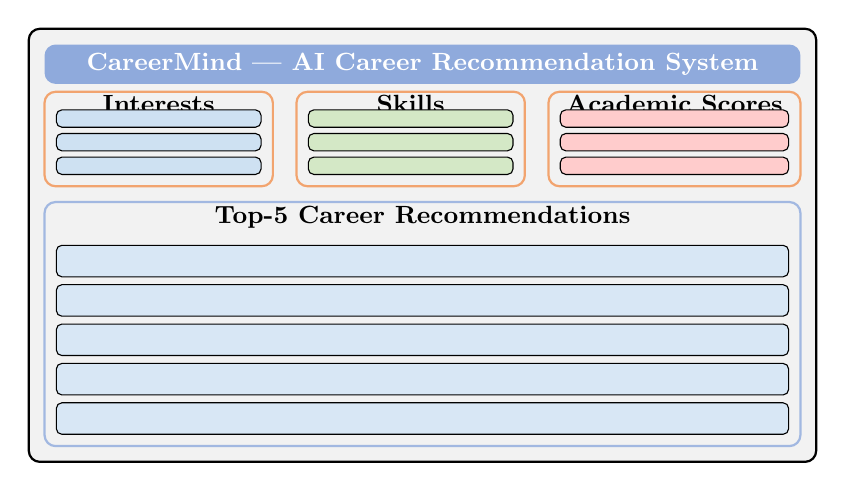
\begin{tikzpicture}
  \draw[thick, rounded corners, fill=gray!10] (0,0) rectangle (10,5.5);
  % Header
  \fill[c1!60, rounded corners] (0.2,4.8) rectangle (9.8,5.3);
  \node[white, font=\bfseries\small] at (5,5.05) {CareerMind — AI Career Recommendation System};
  % Three sections
  \draw[thick, c2!70, rounded corners] (0.2,3.5) rectangle (3.1,4.7);
  \node[font=\small\bfseries] at (1.65,4.55) {Interests};
  \foreach \y in {3.75,4.05,4.35}{
    \draw[fill=c5!50, rounded corners=2pt] (0.35,\y-0.1) rectangle (2.95,\y+0.12);
  }
  \draw[thick, c2!70, rounded corners] (3.4,3.5) rectangle (6.3,4.7);
  \node[font=\small\bfseries] at (4.85,4.55) {Skills};
  \foreach \y in {3.75,4.05,4.35}{
    \draw[fill=c3!50, rounded corners=2pt] (3.55,\y-0.1) rectangle (6.15,\y+0.12);
  }
  \draw[thick, c2!70, rounded corners] (6.6,3.5) rectangle (9.8,4.7);
  \node[font=\small\bfseries] at (8.2,4.55) {Academic Scores};
  \foreach \y in {3.75,4.05,4.35}{
    \draw[fill=c4!20, rounded corners=2pt] (6.75,\y-0.1) rectangle (9.65,\y+0.12);
  }
  % Results
  \draw[thick, c1!50, rounded corners] (0.2,0.2) rectangle (9.8,3.3);
  \node[font=\small\bfseries] at (5,3.1) {Top-5 Career Recommendations};
  \foreach \i in {0,1,2,3,4}{
    \draw[fill=c5!40, rounded corners=2pt]
      (0.35, 0.35+\i*0.5) rectangle (9.65, 0.75+\i*0.5);
  }
\end{tikzpicture}
\caption{Schematic of the CareerMind web interface (input form and results).}
\label{fig:ui-description}
\end{figure}

% =============================================================================
\section{Developer Contributions}
\label{sec:contributions}
% =============================================================================

Table~\ref{tab:contrib} summarises each team member's primary responsibilities.
Figure~\ref{fig:contrib-chart} visualises the approximate percentage share of
total development effort.

\begin{table}[htbp]
\centering
\caption{Developer contributions by module and task.}
\label{tab:contrib}
\begin{tabular}{@{}p{3.5cm}p{4.5cm}c@{}}
\toprule
Developer & Primary Responsibilities & Share (\%) \\
\midrule
Shrushranto Rajbongshi & System architecture, hybrid fusion engine (\texttt{inference.py}), project integration & 25 \\
Priyanshu Mudgal       & Knowledge graph design \& scoring (\texttt{knowledge\_graph.py}), graph edge curation & 20 \\
Aseem Nihal Dang       & Knowledge base development (R01--R66, \texttt{rules.py}), interest \& skill taxonomy & 20 \\
Suraj Pandey           & Neuro-symbolic rule engine (NS01--NS38, \texttt{symbolic\_rules.py}), threshold tuning & 18 \\
Jayesh Solanki         & Flask web application (\texttt{app.py}), HTML/CSS templates, REST API & 17 \\
\bottomrule
\end{tabular}
\end{table}

\begin{figure}[htbp]
\centering
\begin{tikzpicture}
\begin{axis}[
    xbar,
    width=10cm,
    height=6.5cm,
    bar width=0.45cm,
    xmin=0, xmax=30,
    xlabel={Contribution (\%)},
    symbolic y coords={
      {Jayesh Solanki},
      {Suraj Pandey},
      {Aseem Nihal Dang},
      {Priyanshu Mudgal},
      {Shrushranto Rajbongshi}
    },
    ytick=data,
    nodes near coords,
    nodes near coords align={horizontal},
    every node near coord/.append style={font=\small},
    y tick label style={font=\small},
    x tick label style={font=\small},
    xlabel style={font=\small},
    enlarge y limits=0.15,
    grid=major,
    grid style={dashed, gray!40},
    axis line style={thick},
]
\addplot[
    fill=c1,
    draw=c1!80!black
] coordinates {
    (17, {Jayesh Solanki})
    (18, {Suraj Pandey})
    (20, {Aseem Nihal Dang})
    (20, {Priyanshu Mudgal})
    (25, {Shrushranto Rajbongshi})
};
\end{axis}
\end{tikzpicture}
\caption{Developer contribution by percentage of total project effort.}
\label{fig:contrib-chart}
\end{figure}

% =============================================================================
\section{Conclusion and Future Work}
\label{sec:conclusion}
% =============================================================================

This paper presented CareerMind, a hybrid neuro-symbolic expert system for
personalised career recommendation.  By fusing a classic Boolean forward-chaining
layer, a neuro-symbolic layer that blends categorical facts with numeric academic
thresholds, and a multi-hop knowledge graph traversal layer, the system achieves
broad career coverage while producing fully explainable recommendations.
The three-layer fusion formula (Equation~\ref{eq:fusion}) ensures that evidence
from each reasoning paradigm is weighted consistently, eliminating score
inflation when multiple layers agree.

Key empirical findings are: (i)~the knowledge graph layer provides the greatest
coverage, surfacing careers not matched by either rule layer; (ii)~the
neuro-symbolic layer adds discriminative power for borderline academic profiles;
and (iii)~the combination of all three layers yields explanations that users find
more trustworthy than any single-layer output.

\paragraph{Future Directions.}
Several extensions are planned:
\begin{itemize}
  \item \textbf{User feedback loop.}  Collecting explicit ratings on
        recommendations and using them to fine-tune edge weights in the
        knowledge graph via gradient-based optimisation.
  \item \textbf{Expanded career ontology.}  Adding emerging careers
        (e.g.\ Prompt Engineer, Quantum Computing Researcher, Sustainability
        Consultant) and sub-specialisms within existing clusters.
  \item \textbf{Personalised explanation generation.}  Using a language model
        to rephrase rule-level explanations in a tone calibrated to the
        student's academic level.
  \item \textbf{Multi-modal input.}  Incorporating extracurricular activities,
        portfolio artefacts, and personality assessments alongside academic scores.
  \item \textbf{Longitudinal evaluation.}  Tracking whether students who
        followed CareerMind's recommendations report higher career satisfaction
        after graduation.
\end{itemize}

% =============================================================================
\begin{thebibliography}{20}

\bibitem{garcez2022neurosymbolic}
Garcez, A., Lamb, L.C.:
Neurosymbolic AI: The 3rd Wave.
Artificial Intelligence Review \textbf{56}(11), 12387--12406 (2023).
\url{https://doi.org/10.1007/s10462-023-10448-w}

\bibitem{ji2021survey}
Ji, S., Pan, S., Cambria, E., Marttinen, P., Philip, S.Y.:
A Survey on Knowledge Graphs: Representation, Acquisition, and Applications.
IEEE Transactions on Neural Networks and Learning Systems \textbf{33}(2), 494--514 (2022).
\url{https://doi.org/10.1109/TNNLS.2021.3070843}

\bibitem{shortliffe1974mycin}
Shortliffe, E.H.:
MYCIN: Computer-Based Medical Consultations.
Elsevier (1976).

\bibitem{burke2002hybrid}
Burke, R.:
Hybrid Recommender Systems: Survey and Experiments.
User Modeling and User-Adapted Interaction \textbf{12}(4), 331--370 (2002).
\url{https://doi.org/10.1023/A:1021240730564}

\bibitem{chen2018knowme}
Chen, J., Zhang, X., Xu, S.:
KnowMe: A Personalised Career Recommendation System Using a Knowledge Graph.
In: Proc. ACM SIGIR Workshop on ExplainAble Recommendation and Search (2018).

\bibitem{al2019student}
Al-Badarenah, A., Alsakran, J.:
An Automated Recommender System for Course Selection.
International Journal of Advanced Computer Science and Applications \textbf{7}(3), 166--175 (2019).

\bibitem{wang2018ripplenet}
Wang, H., Zhang, F., Wang, J., Zhao, M., Li, W., Xie, X., Guo, M.:
RippleNet: Propagating User Preferences on the Knowledge Graph for Recommender Systems.
In: Proc.\ ACM CIKM 2018, pp.\ 417--426.
\url{https://doi.org/10.1145/3269206.3271739}

\bibitem{wang2019knowledge}
Wang, H., Zhao, M., Xie, X., Li, W., Guo, M.:
Knowledge Graph Convolutional Networks for Recommender Systems.
In: Proc.\ WWW 2019, pp.\ 3307--3313.
\url{https://doi.org/10.1145/3308558.3313417}

\bibitem{mckinlay1999computer}
McKinlay, B., Bloch, D.P.:
DISCOVER: A Computer-Assisted Career Development System.
Journal of Employment Counseling \textbf{27}(2), 73--82 (1990).

\bibitem{katz1993computer}
Katz, M.R.:
Computer-Assisted Career Decision Making: The Guide in the Machine.
Lawrence Erlbaum Associates (1993).

\bibitem{russel2020ai}
Russell, S., Norvig, P.:
Artificial Intelligence: A Modern Approach, 4th edn.
Pearson (2020).

\bibitem{networkx2008}
Hagberg, A., Swart, P., Chult, D.S.:
Exploring Network Structure, Dynamics, and Function using NetworkX.
In: Proc.\ SciPy 2008, pp.\ 11--15.

\bibitem{friedman2001greedy}
Friedman, J.H.:
Greedy Function Approximation: A Gradient Boosting Machine.
The Annals of Statistics \textbf{29}(5), 1189--1232 (2001).

\bibitem{flask2010}
Ronacher, A.:
Flask: A Lightweight WSGI Web Application Framework.
Pallets Projects (2010). \url{https://flask.palletsprojects.com}

\bibitem{guo2020survey}
Guo, Q., Zhuang, F., Qin, C., Zhu, H., Xie, X., Xiong, H., He, Q.:
A Survey on Knowledge Graph-Based Recommender Systems.
IEEE Transactions on Knowledge and Data Engineering \textbf{34}(8), 3549--3568 (2022).
\url{https://doi.org/10.1109/TKDE.2020.3028705}

\end{thebibliography}

\end{document}
